 \documentclass{report}
\usepackage[utf8]{inputenc}
\usepackage[frenchb]{babel}
\usepackage{graphicx}
\usepackage{verbatim}

\title{\textbf{BeaconSandwich} \\ Guide d'utilisation}
\author{Elisoa Ramarokoto \and Thibaud Levasseur \and Guillaume Minette de Saint Martin }
\date{Mars 2015}

\begin{document}

\maketitle
\tableofcontents

\chapter{Première utilisation}

L'application BeaconSandwich ne contient pas encore d'informations lors de son premier lancement.

Pour récupérer ces informations et pouvoir utiliser l'application, il est nécessaire de passer à porté d'un Beacon associé au programme tout en ayant la fonctionnalité Bluetooth de son appareil activé. 

Lorsque l'application détecte le Beacon, elle télécharge automatiquement les flux d'information associés à cette balise. L'ensemble des informations accessibles via ce Beacon sont alors disponibles.

\chapter{Naviguer dans l'application}

\section{Page d'accueil}

Lorsque l'application BeaconSandwich contient des informations en mémoire, celles-ci sont triées par catégorie et disponibles sur la page d'accueil.

Sélectionner une catégorie permet d'afficher les détails et l'ensemble des messages associés.

\begin{figure}[h]
	\centering
	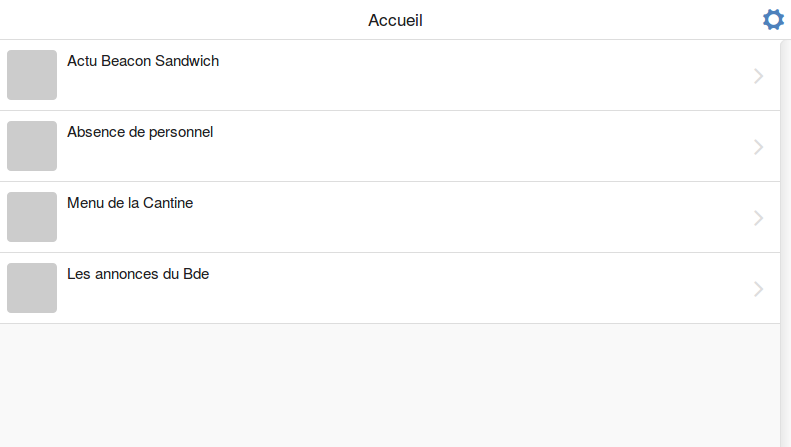
\includegraphics[scale=0.28]{menu.png}
	\caption{Accueil de l'application affichant 4 catégories de flux d'informations}
\end{figure}

\section{Détails d'une catégorie}

Chaque catégorie possède sa propre page avec l'ensemble des messages postés sur l'application. Ces messages sont les communications associés à la catégorie qui ont étés pérédement déposés par d'autres utilisateurs de l'application. Ils peuvent provenir de différentes sources et de dates différentes. 

Un bouton \texttt{Retour} permet de revenir à la page d'accueil.

\begin{figure}[h]
	\centering
	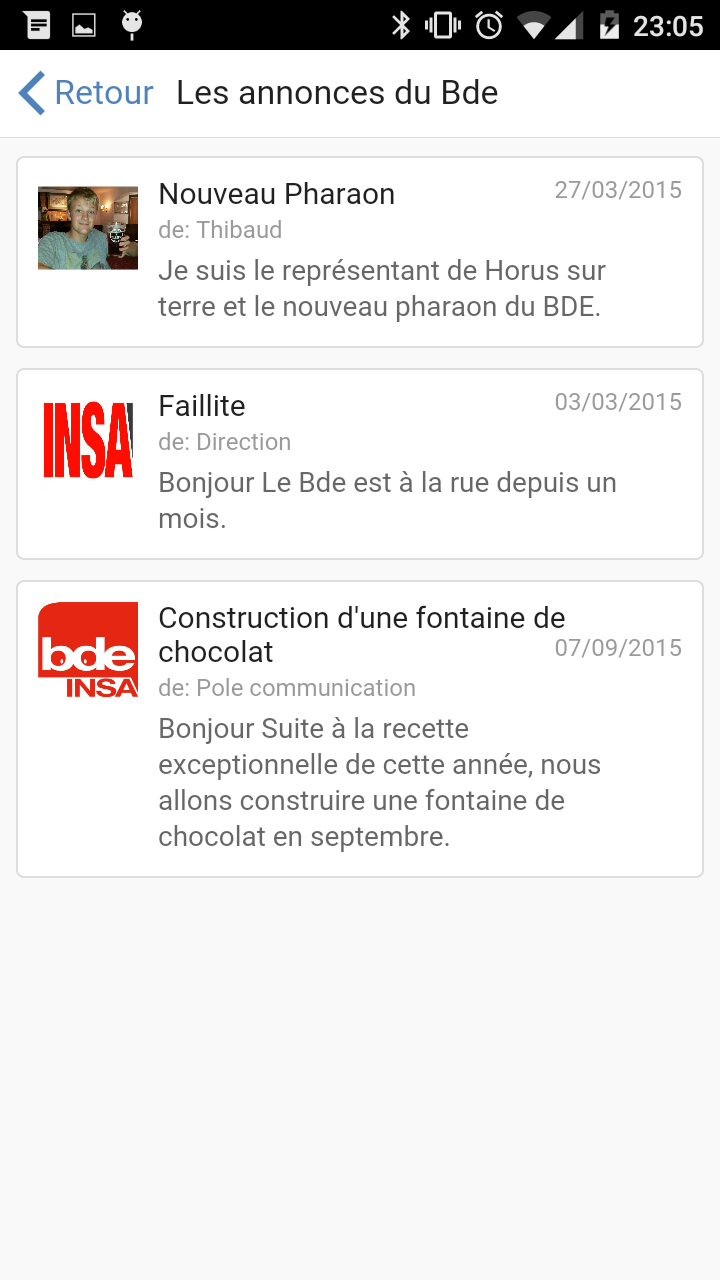
\includegraphics[scale=0.28]{details.png}
	\caption{Détails du flux d'information: \og les annonces du Bde \fg}
\end{figure}

\section{Paramétrage de l'application}

Il est possible de paramétrer les catégories à afficher depuis l'accueil, par la sélection du bouton: 
\includegraphics[scale=0.4]{boutonParam.png}. Un menu affichant l'ensemble des catégories disponibles apparait. Il est alors possible de sélectionner les catégories à afficher à l'écran d'accueil.

Un bouton \texttt{Retour} permet de revenir à la page d'accueil.


\begin{figure}[h]
	\centering
	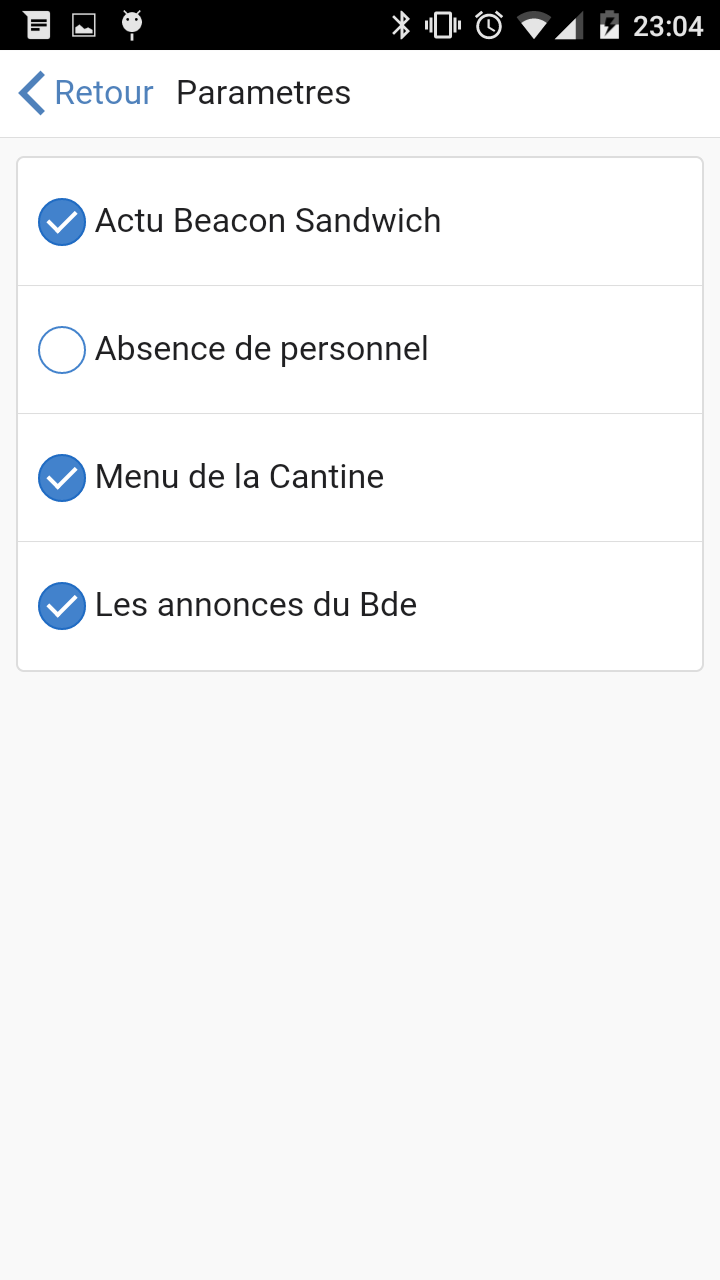
\includegraphics[scale=0.28]{parametres.png}
	\caption{Paramètrage de l'application pour ne plus afficher la catégorie \og Absence de personnel \fg}
\end{figure}

\begin{figure}[h]
	\centering
	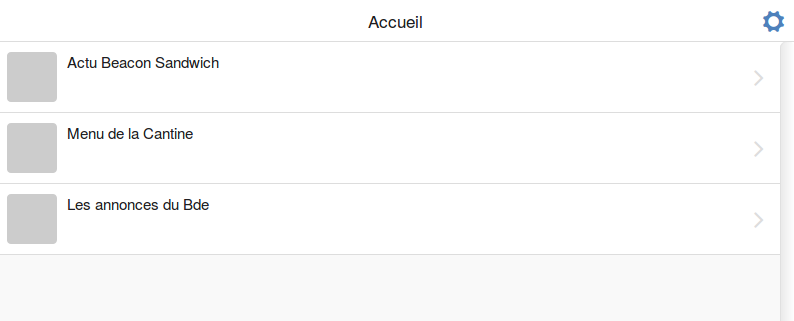
\includegraphics[scale=0.28]{accueilPerso.png}
	\caption{La page d'accueil après déselection de la catégorie \og Absence de personnel \fg}
\end{figure}

\chapter{Gestion des flux d'information}

\section{Avant propos}

Les catégories ainsi que les messages associés sont téléchargés dans l'application depuis un serveur en ligne associé au Beacon à portée. 

C'est à dire que chacun peut, à l'aide d'un Beacon et d'un serveur, ajouter des informations que l'application affichera lorsqu'elle reconnaîtra la balise.

\section{Ajouter des informations}

Les catégories, ainsi que les messages sont stockées dans un fichier \texttt{xml} sur le serveur puis interprétées et enregistrées dans l'application. Chaque Beacon est donc lié à une page internet permettant le téléchargement d'un fichier de données.
Ce fichier \texttt{xml} est téléchargé depuis le serveur dès la détection du Beacon par l'application.

Le fichier utilisé pour les exemples de ce manuel est disponible en annexe et peut servir de modèle pour la structure d'un autre fichier \texttt{xml} de stockage de données.


\chapter{Annexe}

\section*{Exemple de fichier \texttt{xml} de définition d'informations}
\begin{verbatim}
<listedeflux>

	<flux>
		<nom>Les annonces du Bde</nom>
		<listedemessages>

			<message>
				<source>Pole communication</source> <titre>Construction d'une fontaine de chocolat</titre> <date>07/09/2015</date><uuid>ABC00000-0000-0000-0000-000000000000</uuid>
				<infos>
					Bonjour
					Suite à la recette exceptionnelle de cette année, nous allons construire une fontaine de chocolat en septembre.
				</infos>
				<priorite>
					1
				</priorite>
			</message>

			<message>
				<source>Direction</source> <titre>Faillite</titre> <date>03/03/2015</date><uuid>ABC00000-0000-0000-0000-000000000000</uuid>
				<infos>
					Bonjour
					Le Bde est à la rue depuis un mois.
				</infos>
				<priorite>
					2
				</priorite>
			</message>
			<message>
				<source>Thibaud</source> <titre>Nouveau Pharaon</titre> <date>27/03/2015</date><uuid>ABC00000-0000-0000-0000-000000000000</uuid>
				<infos>
					Je suis le représentant de Horus sur terre et le nouveau pharaon du BDE.
				</infos>
				<priorite>
					2
				</priorite>
			</message>
		</listedemessages>
	</flux>

	<flux>
		<nom>Menu de la Cantine</nom>
		<listedemessages>

			<message>
				<source>Monique de la cuisine</source> <titre>Menu de demain</titre> <date>07/02/2015</date> <uuid>ABCD0000-0000-0000-0000-000000000000</uuid>
				<infos>
					Bonjour
					Ce mardi, nous aurons pour déjeuner du poulet aux olives.
				</infos>
				<priorite>
					1
				</priorite>
			</message>

			<message>
				<source>Monique de la cuisine</source> <titre>Menu de ce midi</titre> <date>02/03/2015</date> <uuid>ABCD0000-0000-0000-0000-000000000000</uuid>
				<infos>
					Bonjour
					Ce lundi, nous aurons pour déjeuner du boudain noir.
				</infos>
				<priorite>
					1
				</priorite>
			</message>

		</listedemessages>
	</flux>

	<flux>
		<nom>Absence de personnel</nom>
		<listedemessages>

			<message>
				<source>Secrétariat</source> <titre>Absence de Mme Dupond</titre> <date>07/02/2015</date> <uuid>00002</uuid>
				<infos>
					Bonjour
					Mme Dupond sera absente aujourd'hui.
				</infos>
				<priorite>
					1
				</priorite>
			</message>

		</listedemessages>
	</flux>
</listedeflux>

\end{verbatim}

\end{document}